\documentclass[12pt,a4paper]{article}
\usepackage{tikz}
\usetikzlibrary{trees}
\usepackage{amsmath}
\usepackage{forest}
\usepackage{commons/course}


%\hidesolutions



\شروع{نوشتار}
\سربرگ{}{آزمون پایان‌ترم}{25 خرداد ۱۳۹8}{}

\vspace*{-2in}
\begin{center}
	به نام او
\end{center}
\vspace*{1.5in}
- امتحان از 120 نمره می‌باشد و نمره کامل این امتحان، 90 می‌باشد.\\
- هر سوال را در یک صفحه جدا پاسخ دهید و مشخصات خود را در هر صفحه بنویسید.\\
- طراح سوالات: دکتر شریفی، علیرضا اکبری، شبنم شیخها، پدرام خورسندی، آراد محمدی، آریا کوثری، امیر مجتبی صبور و متین خواجوی\\
\vspace*{-0.5in}
\section*{سوالات کوتاه‌پاسخ (30 نمره)}
\شروع{ابجد}

\فقره درستی یا نادرستی عبارت زیر را مشخص کنید. جواب خود را توجیه کنید.(10نمره)
\شروع{فقرات}
\فقره صحیح. \\
در چنین آرایه‌ای تعداد نابجایی‌ها حداکثر 
$200n$
تاست، زیرا عناصری که جابجا نمی‌شوند با هم‌دیگر نابجایی ندارند. در ۱۰۰ عمل جابجایی، ۲۰۰ عنصر با هم جابجا می‌شوند که این ۲۰۰ عنصر هر کدام حداکثر با $n$ عنصر دیگر نابجایی دارند. می‌دانیم که الگوریتم
\lr{sort insertion}
به تعداد نابجایی‌ها عملیات انجام می‌دهد، پس با این الگوریتم می‌توان آرایه را در زمان $O(n)$ مرتب کرد. 

\فقره صحیح. \\
اگر اعداد را به مبنای $n$ ببریم هر عدد به یک عدد دورقمی تبدیل می‌شود. حال می‌توان این اعداد را با
\lr{sort radix}
در $O(n)$ مرتب کرد. 

\فقره غلط. \\
عنصر بعدی در زیردرخت فرزند راست قرار دارد. تمامی عناصر زیردرخت فرزند راست این رأسِ، از آن بزرگ‌ترند. کوچک‌ترین این عناصر، یعنی چپ‌ترین عنصر با شروع از ریشه، عنصر بعدی این رأس است. پس عنصر بعدی، 
\textit{فرزند چپ}
نباید داشته باشد و فرزند راست داشتنِ آن مشکلی ایجاد نمی‌کند. به همین ترتیب می‌توان برای عنصر قبلی استدلال کرد. 

\فقره غلط. \\
دو د.د.ج زیر را در نظر بگیرید. تعداد راه‌های ساختن سمت راست ۴ و سمت چپ ۱ است. برای همین احتمال ساختن د.د.ج سمت راست ۴ برابر ساختن د.د.ج سمت چپ است. در حالی که اگر همه‌ی درختان با ۵ گره را در نظر بگیریم و از بین آن‌ها یکی را انتخاب کنیم، احتمال انتخاب د.د.ج سمت راست با د.د.ج سمت چپ برابر است. 
\begin{figure}[h!]
	\centering
	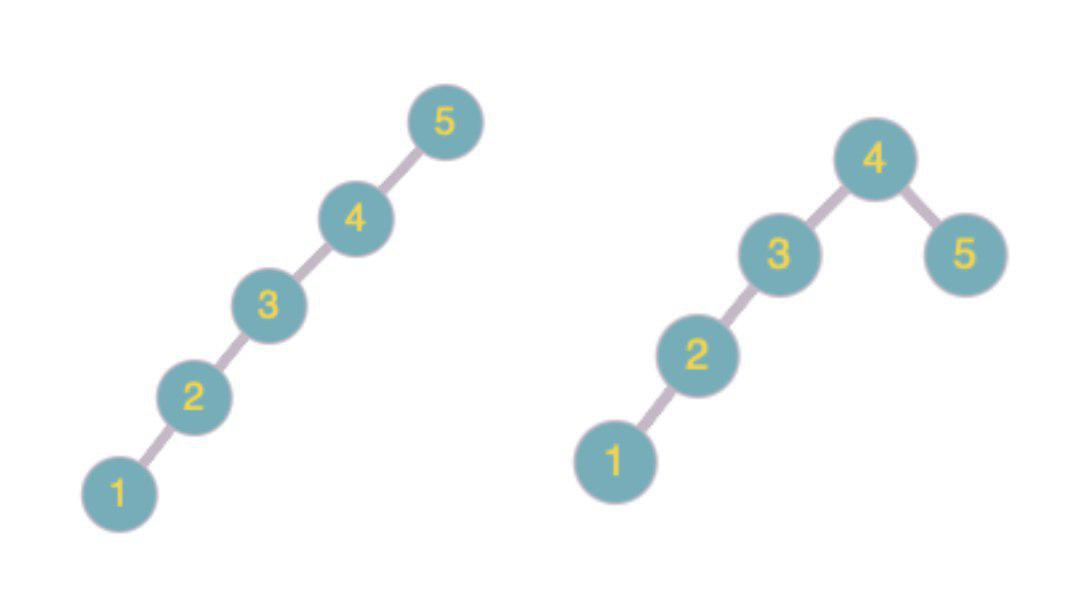
\includegraphics[width=0.4\linewidth]{figs/tree}
\end{figure}

\newpage
\پایان{فقرات} 
\فقره از الگوریتمی استفاده می‌کنیم که در هر مرحله، راس با درجه ورودی صفر را پیدا می‌کند و آن راس و یالهای خروجی آنرا از گراف حذف می‌کند و این عملیات را به‌صورت \lr{iterative} انجام می‌دهد.\\
لم: در یک \lr{DAG} همواره حداقل یک راس با درجه ورودی صفر وجود دارد. \\
با توجه به لم، در هر مرحله الگوریتم، اگر راس با درجه ورودی صفر دیگر موجود نبود، یعنی گراف دور دارد. در غیر اینصورت ترتیب توپولوژیکال بدست می‌آید.

\فقره پیچیدگی زمانی به ترتیب: $O(n log n)$ و $O(n^3)$
\پایان{ابجد}

\مسئله{مَمَّد در فینال لیگ قهرمانان اروپا(20 نمره)}
- کوچکترین عضو در خانه [1,1] قرار دارد. حال این مقدار را خارج می‌کنیم و به جای آن $\infty$ می‌گذاریم. در ادامه برای بر قراری خاصیت جدول، $\infty$ را با کمینه دو خانه [1,2] یا [2,1] جایگزین می‌کنیم. حال مسئله ما به یک جدول $(m-1) \times n$ و یا $m \times (n-1)$ تبدیل می‌شود. پیچیدگی زمانی نیز از $O(m+n)$ می‌باشد زیرا حداکثر $3(m+n)$ عمل انجام می‌دهیم.

- در خانه \lr{[m,n]} بیشترین مقدار قرار دارد. در آن جا درج کرده و با عملیاتی مانند بخش قبل، عضو جدید را در جای درستش قرار می‌دهیم.
\\
- از آنجایی که در جدول قرار دارند، کافیست $n^2$ بار تابع بخش قبل را صدا بزنیم.

\مسئله{واسه همه پیگیری‌هات مرسی(15 نمره)}
اگر $G$ یک درخت باشد، با توجه به این که $T_1$ و $T_2$ هر دو درخت هستند باید دارای تمامی یال‌های $G$ باشند پس با هم برابر هستند.

برای ثابت کردن این که $G$ یک درخت است اگر $T_1$ و $T_2$ برابر باشند، از برهان خلف استفاده می‌کنیم و فرض خلف می‌کنیم که $G$ درخت نباشد. در این صورت $G$ حداقل حاوی یک دور به نام $C$ است که راس‌های آن  را به ترتیب دور $u_1$ تا $u_k$ می‌نامیم. 

در $T_2$ هر $u_i$ و $u_{i+1}$ ای که در نظر بگیریم (و همچنین $u_k$ و $u_1$) یکی از آنها باید جد آن یکی باشد. زیرا در غیر این صورت (اگر آن که زودتر پیمایش شده $u_i$ باشد)، باید قبل از این که الگوریتم از $u_i$ خارج شود، $u_{i+1}$  پیمایش شود وگرنه با یال مستقیم $u_i$ به $u_{i+1}$ الگوریتم جستجوی عمق اول وارد آن می‌شد (پس به هر حال$u_{i+1}$ در زیردرخت $u_i$ است). پس تمامی رئوس $C$ در یک مسیر از ریشه به برگ در $T_2$ قرار دارند.

اما در اولین جایی که الگوریتم جستجوی سطح اول به راسی از $C$ به نام $u_j$ می‌رسد، اگر $u_{j-1}$ و $u_{j+1}$ قبلا علامت‌گذاری نشده‌باشند، همانجا دو شاخه برای رئوس $C$  در $T_1$ تولید می‌شود و اگر حداقل یکی از آنها از قبل علامت‌گذاری شده باشد، از قبل دو شاخه تولید شده‌اند (که یکی به $u_j$ رسیده و دیگری به یکی از همسایه‌هایش). پس تمامی رئوس $C$ در یک مسیر از ریشه به برگ در $T_1$ قرار نخواهند داشت. پس $T_1$ با $T_2$ متقاوت خواهد بود و فرض خلف باطل و حکم ثابت می‌شود.

\newpage
\مسئله {مسیریابی(15 نمره)}
شرایط قسمت الف یک گراف بدون وزن است بنابراین می‌توان به سادگی با الگوریتم \lr{BFS} این مسیر را پیدا کرد

در قسمت ب نیز با تغییر اندکی در الگوریتم \lr{Dijkstra} می‌توانیم به جواب برسیم. فرض کنیم مقدار کوتاه‌ترین فاصله‌ی هر راس را تا مبدا در آرایه‌ی $d$ ذخیره کرده‌ایم (همان آرایه‌ای که در طول الگوریتم تغییر می‌کند و در هر مرحله راس با کمترین مقدار $d$ را به مجموعه $S$ اضافه می‌کنیم). اگر بتوانیم در زمان $t$ به راس $x$ برسیم، در هنگام به روز رسانی آرایه ی برای همسایگان $x$ (مثلا راس $y$ با وزن یال $w$) دیگر زمان رسیدن به $y$ از طریق راس $x$ برابر با $d_x + w$  نخواهد بود؛ بلکه برابر با $d_x + T_x + w$ است و باید این مقدار را با مقدار کنونی $d_y$ مقایسه کنیم. البته برای راس شروع این قضیه برقرار نیست و این موضوع را باید «دستی» چک کنیم! هزینه زمانی این الگوریتم هم عیناً مانند الگوریتم دایکسترا است.


\مسئله{پیش از تابستان\footnote{به تقلید از سه‌گانه "پیش از" اثر ریچارد لینکلیتر}(20 نمره)}

رشته مورد نظر را هش می کنیم.ابتدا بلند ترین رشته ای را میبایم که هم پیشوند $A$ باشد و هم پسوند $A$ باشد.(این کار را به این صورت انجام می دهیم که به ازای هر طول رشته مانند $t$ با مقایسه هش ها ، می توانیم در $O(1)$ بفهمیم که رشته ی به طول $t$ به صورت پیشوند و پس وند ظاهر شده است یا نه).بعد از اینکه بلند ترین رشته را به دست آوردیم که هم پیشوند باشد هم پسوند، میتوانیم با الگوریتمی از $O(n)$ بفهمیم که این رشته به صورت میانوند ظاهر شده است یا خیر(با طی کردن کل رشته و مقایسه هش آن) اگر این رشته پیدا شده، به صورت میانوند نیز ظاهر شده بود، جواب ما پیدا شده است در غیر این صورت ، دومین بلند ترین زیر رشته که هم به صورت پیشوند آمده و هم به صورت پسوند، قطعا جواب مسئله است به صورت زیر:
\\
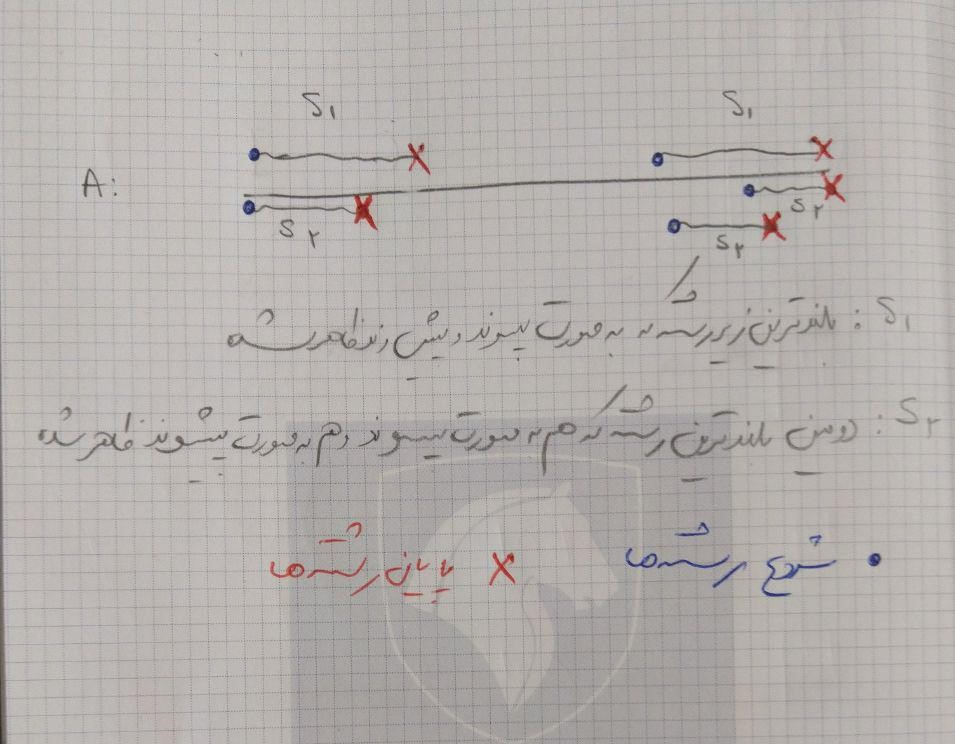
\includegraphics[width = \linewidth]{figs/1.jpg}\\

\newpage
\مسئله{سَم(20 نمره)}
ایده این سوال استفاده از \lr{binary search} می‌باشد. نکته دیگر این است اگر سر مار در مستطیل ما باشد جوابی که می‌گیریم فرد می‌باشد. 
\\
حال کافیست هر بار نصف بخشی از تالاب را که جستجو نکرده‌ایم، بررسی کنیم و اگر جواب فرد بود همان بخش را ادامه می‌دهیم و در غیر این صورت، نصفه دیگر را. این کار را ادامه می‌دهیم تا در نهایت سر مار پیدا شود.


\پایان{نوشتار}
